\documentclass{report}


\usepackage[T1]{fontenc}
\usepackage[utf8]{inputenc}
\usepackage{amsmath}


\usepackage{enumerate}

\usepackage{graphicx}
\usepackage{fancyhdr}
\usepackage{lettrine}
\usepackage{hyperref}
\usepackage{subcaption}
\usepackage{tikz}
\usepackage{cite}
\usepackage{listings}
\usepackage[nottoc, numbib]{tocbibind}
\usepackage{../assets/scripts/tex/color-env}
\usepackage[ngerman]{babel}
\usepackage[Glenn]{fncychap}
\usepackage{trfsigns}
\usepackage{amsmath,amsfonts,stmaryrd,amssymb} % Math packages

\usepackage{enumerate} % Custom item numbers for enumerations

\usepackage[ruled]{algorithm2e} % Algorithms

\usepackage[]{mdframed} % Allows defining custom boxed/framed environments


\mdfdefinestyle{info}{%
	topline=false, bottomline=false,
	leftline=false, rightline=false,
	nobreak,
	singleextra={%
		\fill[black](P-|O)circle[radius=0.4em];
		\node at(P-|O){\color{white}\scriptsize\bf i};
		\draw[very thick](P-|O)++(0,-0.8em)--(O);%--(O-|P);
	}
}

% Define a custom environment for information
\newenvironment{info}[1][Info:]{ % Set the default title to "Info:"
	\medskip
	\begin{mdframed}[style=info]
		\noindent{\textbf{#1}}
}{
	\end{mdframed}
}


\mdfdefinestyle{warning}{
	topline=false, bottomline=false,
	leftline=false, rightline=false,
	nobreak,
	singleextra={%
		\draw(P-|O)++(-0.5em,0)node(tmp1){};
		\draw(P-|O)++(0.5em,0)node(tmp2){};
		\fill[black,rotate around={45:(P-|O)}](tmp1)rectangle(tmp2);
		\node at(P-|O){\color{white}\scriptsize\bf !};
		\draw[very thick](P-|O)++(0,-1em)--(O);%--(O-|P);
	}
}

% Define a custom environment for warning text
\newenvironment{warn}[1][Warning:]{ % Set the default warning to "Warning:"
	\medskip
	\begin{mdframed}[style=warning]
		\noindent{\textbf{#1}}
}{
	\end{mdframed}
}


\usetikzlibrary{shapes}
    \usetikzlibrary{arrows}
    \usetikzlibrary{arrows.meta,topaths}
    \usetikzlibrary{bending}
    \usetikzlibrary{calc}
\title{Elektrotechnik 1 Praktikum 1}


\usepackage[
  includehead,
  headheight = 17mm,
  footskip = \dimexpr\headsep+\ht\strutbox\relax,
  tmargin = 0mm,
  bmargin = \dimexpr17mm+2\ht\strutbox\relax,
]{geometry}

\usepackage{anyfontsize}
\usepackage{float}
\usepackage{xcolor}

\definecolor{DarkGreenBlue}{HTML}{264653}
\definecolor{LightGreenBlue}{HTML}{2A9D8F}
\definecolor{LightOrange}{HTML}{E9C46A}
\definecolor{DarkOrange}{HTML}{F4A261}
\definecolor{RedOrange}{HTML}{E76F51}
\definecolor{BrightRed}{HTML}{D62828}
\definecolor{DeepBlue}{HTML}{003049}

\lstdefinestyle{code}{
    backgroundcolor=\color{backcolour},
    commentstyle=\color{codegreen},
    keywordstyle=\color{magenta},
    numberstyle=\tiny\color{codegray},
    stringstyle=\color{codepurple},
    basicstyle=\ttfamily\footnotesize,
    breakatwhitespace=false,
    breaklines=true,
    captionpos=b,
    keepspaces=true,
    numbers=left,
    numbersep=5pt,
    showspaces=false,
    showstringspaces=false,
    showtabs=false,
    tabsize=2
}

\definecolor{codegreen}{rgb}{0,0.6,0}
\definecolor{codegray}{rgb}{0.5,0.5,0.5}
\definecolor{codepurple}{rgb}{0.502,0.502,0.0}
\definecolor{backcolour}{rgb}{0.95,0.95,0.95}

\lstdefinelanguage{ST}
{
	morekeywords={
	case,of,if,then,end_if,end_case,super,function_block,extends,var,
	constant, byte,,end_var,var_input, real,bool,var_output,
	dint,udint,word,dword,array, of,uint,not,adr, program, for, end_for, while, do, end_while, repeat, end_repeat, until, to, by, else, elsif
	},
	otherkeywords={
		:, :=, <>,;,\,.,\[,\],\^,1,2,3,4,5,6,7,8,9,0, TRUE, FALSE, \{attribute,  \'hide\'\}
	},
	keywords=[1]{
		case,of,if,then,end_if,end_case,super,function_block,extends,var,
		constant, byte,,end_var,var_input, real,bool,var_output,
		dint,udint,word,dword,array, of,uint,not,adr, :, :=, <>,;,\,.,\[,\],\^,program, for, end_for, while, do, end_while, repeat, end_repeat, until, to, by, else, elsif
	},
	keywordstyle=[1]\color{blue},
	keywords=[2]{
		1,2,3,4,5,6,7,8,9,0, TRUE, FALSE
	},
	keywordstyle=[2]\color{codepurple},
	keywords=[3]{
		\{attribute,  \'hide\'\}
	},
	keywordstyle=[3]\color{codegray},
	sensitive=false,
	morecomment=[l]{//},
	morecomment=[s]{(*}{*)},
	morestring=[b]"
	morestring=[b]'
}

\lstset{
	language={ST},
	backgroundcolor=\color{backcolour},
	commentstyle=\color{codegreen}\textit,
	keywordstyle=\color{blue},
	numberstyle=\tiny\color{codegray},
	stringstyle=\color{codepurple},
	basicstyle=\ttfamily\scriptsize,
	breakatwhitespace=false,
	breaklines=true,
	captionpos=b,
	keepspaces=true,
	numbers=left,
	numbersep=5pt,
	showspaces=false,
	showstringspaces=false,
	showtabs=false,
	tabsize=2
}
\pagestyle{fancy}
\fancyhead[L]{\leftmark}
\fancyhead[R]{}
\fancyfoot[L]{}
\fancyfoot[C]{\thepage}
\fancyfoot[R]{
\includegraphics[scale=0.2]{../assets/images/haw.jpg}}
\renewcommand\headrulewidth{0.5pt}


\begin{document}


\thispagestyle{empty}
\begin{tikzpicture}[overlay,remember picture]
  \thispagestyle{empty}
  \fill[black!2] (current page.south west) rectangle (current page.north east);

  \begin{scope}[transform canvas ={rotate around ={45:($(current page.north west)+(-.5,-6)$)}}]

    \shade[rounded corners=18pt, left color=DarkGreenBlue, right color=LightGreenBlue] ($(current page.north west)+(-.5,-6)$) rectangle ++(9,1.5);

  \end{scope}

  \begin{scope}[transform canvas ={rotate around ={45:($(current page.north west)+(.5,-10)$)}}]

    \shade[rounded corners=18pt, left color=LightOrange,right color=DarkOrange] ($(current page.north west)+(0.5,-10)$) rectangle ++(15,1.5);

  \end{scope}

  \begin{scope}[transform canvas ={rotate around ={45:($(current page.north west)+(0.5,-10)$)}}]

    \shade[rounded corners=8pt, right color=DarkOrange, left color=LightOrange] ($(current page.north west)+(1.5,-9.55)$) rectangle ++(7,.6);

  \end{scope}

  \begin{scope}[transform canvas ={rotate around ={45:($(current page.north)+(-1.5,-3)$)}}]

    \shade[rounded corners=12pt, left color=DeepBlue!80, right color=DeepBlue!60] ($(current page.north)+(-1.5,-3)$) rectangle ++(9,0.8);

  \end{scope}

  \begin{scope}[transform canvas ={rotate around ={45:($(current page.north)+(-3,-8)$)}}]

    \shade[rounded corners=28pt, left color=BrightRed, right color=BrightRed!80] ($(current page.north)+(-3,-8)$) rectangle ++(15,1.8);

  \end{scope}

  \begin{scope}[transform canvas ={rotate around ={45:($(current page.north west)+(4,-15.5)$)}}]

    \shade[rounded corners=25pt, left color=RedOrange, right color=DarkOrange] ($(current page.north west)+(4,-15.5)$) rectangle ++(30,1.8);

  \end{scope}

  \begin{scope}[transform canvas ={rotate around ={45:($(current page.north west)+(13,-10)$)}},]

    \shade[rounded corners=22pt, left color=DeepBlue,right color=DarkGreenBlue] ($(current page.north west)+(13,-10)$) rectangle ++(15,1.5);

  \end{scope}

  \begin{scope}[transform canvas ={rotate around ={45:($(current page.north west)+(18,-8)$)}},]

    \shade[rounded corners=8pt, left color=DarkOrange] ($(current page.north west)+(18,-8)$) rectangle ++(15,0.6);

  \end{scope}

  \begin{scope}[transform canvas ={rotate around ={45:($(current page.north west)+(19,-5.65)$)}},]

    \shade[rounded corners=12pt, left color=RedOrange] ($(current page.north west)+(19,-5.65)$) rectangle ++(15,0.8);

  \end{scope}

  \begin{scope}[transform canvas ={rotate around ={45:($(current page.north west)+(20,-9)$)}}]

    \shade[rounded corners=20pt, left color=BrightRed, right color=BrightRed!80] ($(current page.north west)+(20,-9)$) rectangle ++(14,1.2);

  \end{scope}

  \draw[ultra thick,gray] ($(current page.center)+(5,2)$) -- ++(0,-3cm) node[midway,left=0.25cm,text width=5cm,align=right,black!75]{{\fontsize{25}{30} \selectfont \bf RT\\[10pt] Bericht}} node[midway,right=0.25cm,text width=6cm,align=left,orange]{{\fontsize{70}{86} \selectfont 2021}};

  \node at ($(current page.center)+(0,-4)$) {{\fontsize{40}{72} \selectfont Regelungstechnik}};

  \node[text width=8cm,align=center] at ($(current page.center)+(0,-6.5)$) {{\fontsize{16}{20} \selectfont \textcolor{orange}{ \bf \today}} \\[3pt] Florian Tietjen 2519584\\[3pt] Emily Antosch 2519935};

\end{tikzpicture}

\newpage

\tableofcontents

\listoffigures

\newpage

\chapter{SIPN mit ST}

\section{Einführung}
\label{sec:einfuhrung}

Im nächsten Teil des Labors wollen wir uns mit dem Lager und dem Transportarm beschäftigen. Dieses Mal verwenden wir dafür allerdings die Programmiersprache ST und das Prinzip von Steuerungstechnisch interpretierten Petrinetzen (SIPN). Wir wollen einen steuerungstechischen Ablauf erstellen, bei dem in einer dauerhaften Schleife, die Werkstücke vom Lager zum Band transportiert werden, um dort weiter verarbeitet zu werden.

\section{Vorbereitung}

Wir wollen uns zunächst mit dem Petrinetz befassen, welches wir dann dazu verwenden wollen, einen Teil der Steuerungsstrecke in ST zu programmieren. Das Petrinetz enthält, wie in den Anforderungen genannt, nur den Automatikmodus der Anlage. Der Betriebkopf zum Umschalten wird erst im folgenden Praktikum behandelt und ist daher nur schematisch durch Schreiben der Variablen beim Debuggen der Anlage in CodeSYS umgesetzt.


\begin{figure}[H]
  \centering
  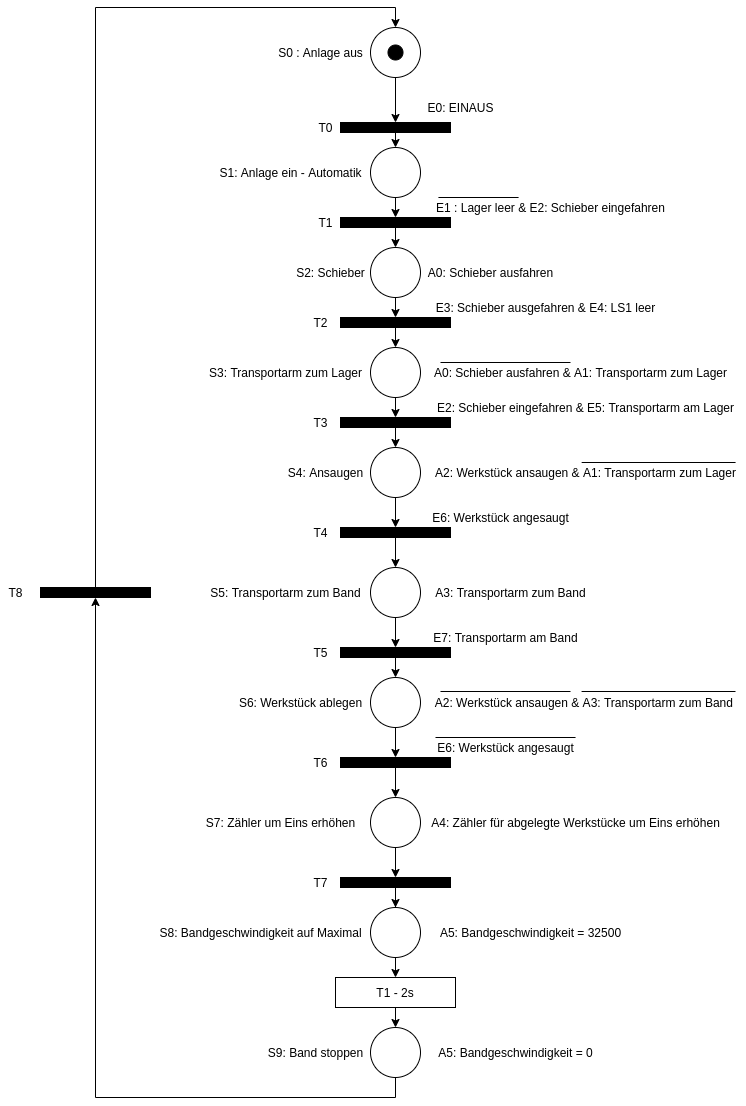
\includegraphics[width=\textwidth]{../assets/images/ST2/petrinetz.png}
  \caption{Petrinetz für den Automatikmodus der Anlage}
\label{fig:petrinetz}
\end{figure}
\newpage
Wie oben zu sehen ist, haben wir den Ablauf der technischen Anforderungen umgesetzt. In einer laufenden Schleife, wird zunächst der Schieber mit einem Werkstück ausgefahren und dann von dem Transportarm abgeholt, solange in der Pufferstrecke Platz ist. Im Anschluss saugt der Arm das Werkstück an und transportiert dieses zum Band, um es dort wieder loszulassen. Der Zähler für die abgelegt, das Band wird für 2 Sekunden auf der maximalen Geschwindigkeit bewegt und kommt dann zum Stehen, woraufhin der Ablauf von vorne anfängt. Wurde an irgendeinem Punkt die EINAUS-Funktion auf AUS gestellt, wird Sie genau an diesem Punkt umgesetzt und die Anlage ist außer Betrieb.

\section{Programmierung der Anlage in ST durch SIPN}

Wir haben den folgenden Code in ST für die Steuerung der Anlage verwendet

\begin{lstlisting}
VAR_INPUT
    ls1: BOOL; (* Lichtschranke 1 leer *)
    piece_sucked: BOOL; (* Werkstueck angesaugt *)
    storage_empty: BOOL; (* Lagerplatz leer *)
    piston_extended: BOOL; (* Piston ausgeklappt *)
    piston_reduced: BOOL; (* Piston eingeklappt *)
    arm_at_storage: BOOL; (* Arm am Lagerplatz *)
    arm_at_band: BOOL; (* Arm am Band *)
END_VAR
VAR_OUTPUT
    band_speed: WORD; (* Bandgeschwindigkeit auf Hardware *)
    extend_piston : BOOL (* Ausschieber auf Hardware ausfahren *)
    arm_to_lager : BOOL (* Arm zum Lager auf Hardware fahren *)
    arm_to_band : BOOL (* Arm zum Band auf Hardware fahren *)
    suck_piece : BOOL (* Werkstueck angesaugt *)
    release_piece : BOOL (* Werkstueck loslassen *)
END_VAR
VAR
    S0 : BOOL := TRUE (* Initialisierung des Startzustands*)
    S1, S2, S3, S4, S5, S6, S7, S8, S9 : BOOL; (* Zustaende *)
    counter : WORD; (* Zaehler fuer abgelegte Werkstuecke *)
    counter_FP : BOOL; (* Flankendetektion fuer Zaehler *)
    counter_FHM : BOOL; (* Flankendetektion fuer Zaehler *)
    EINAUS: BOOL; (* Ein/Aus *)
    AUTOMAN: BOOL := 1; (* Automatisch/Manuell *)
    HAND_BAND_EIN: BOOL; (* Transportband bewegen/stoppen *)
    HAND_BANDV: WORD; (* Transportband Geschwindigkeit *)
    HAND_AUSSCHIEBER: BOOL; (* Ausschieber aktiv *)
    HAND_ARM_ZUM_LAGER: BOOL; (* Arm zum Lager *)
    HAND_ARM_ZUM_BAND: BOOL; (* Arm zum Band *)
    HAND_ANSAUGEN: BOOL; (* Werkstueck ansaugen *)
    HAND_LOSLASSEN: BOOL; (* Werkstueck loslassen *)
    T1 : TON; (* Timer fuer Band *)
END_VAR
IF AUTOMAN THEN
    WHILE EINAUS DO
        IF (S0 AND NOT S1 AND EINAUS) THEN
            S1 := TRUE;
            S0 := FALSE;
        END_IF;
        IF (S1 AND NOT S2 AND NOT storage_empty AND piston_reduced) THEN
            S2 := TRUE;
            S1 := FALSE;
        END_IF;
        IF (S2 AND NOT S3 AND piston_extended AND ls1) THEN
            S3 := TRUE;
            S2 := FALSE;
        END_IF;
        IF (S3 AND NOT S4 AND arm_at_storage AND piston_reduced) THEN
            S4 := TRUE;
            S3 := FALSE;
        END_IF;
        IF (S4 AND NOT S5 AND piece_sucked) THEN
            S5 := TRUE;
            S4 := FALSE;
        END_IF;
        IF (S5 AND NOT S6 AND arm_at_band) THEN
            S6 := TRUE;
            S5 := FALSE;
        END_IF;
        IF (S6 AND NOT S7 AND NOT piece_sucked) THEN
            S7 := TRUE;
            S6 := FALSE;
        END_IF;
        IF (S7 AND NOT S8 AND T1.Q) THEN
            S8 := TRUE;
            S7 := FALSE;
            band_speed := 32500;
        END_IF;
        IF (S8 AND NOT S9) THEN
            S9 := TRUE;
            S8 := FALSE;
            band_speed := 0;
        END_IF;
        IF (S9 AND NOT S0) THEN
            S0 := TRUE;
            S9 := FALSE;
        END_IF;
        extend_piston := S2;
        arm_to_lager := S3;
        suck_piece := S4 OR S5;
        arm_to_band := S5;
        release_piece := S6;
        counter_FP := S7 and NOT counter_FHM;
        counter_FHM := S7;
        IF counter_FP THEN
            counter := counter + 1;
        END_IF;
        IF S8 THEN
            band_speed := 32500;
        ELSE
            band_speed := 0;
        END_IF;
        T1(IN:=S7 AND NOT S8, PT:=T#2s);
    END_WHILE;
ELSE
    IF EINAUS THEN
        IF HAND_BAND_EIN THEN
            band_speed := HAND_BANDV;
        ELSE
            band_speed := 0;
        END_IF;

        IF HAND_AUSSCHIEBER THEN
            extend_piston := TRUE;
        ELSE
            extend_piston := FALSE;
        END_IF;

        IF HAND_ARM_ZUM_LAGER AND NOT HAND_ARM_ZUM_BAND THEN
            arm_to_lager := TRUE;
        ELSE
            arm_to_lager := FALSE;
        END_IF;

        IF HAND_ARM_ZUM_BAND AND NOT HAND_ARM_ZUM_LAGER THEN
            arm_to_band := TRUE;
        ELSE
            arm_to_band := FALSE;
        END_IF;

        IF HAND_ANSAUGEN AND NOT HAND_LOSLASSEN THEN
            suck_piece := TRUE;
        ELSE
            suck_piece := FALSE;
        END_IF;

        IF HAND_LOSLASSEN AND NOT HAND_ANSAUGEN THEN
            release_piece := TRUE;
        ELSE
            release_piece := FALSE;
        END_IF;
    END_IF;
END_IF;
\end{lstlisting}

\end{document}
